\documentclass{standalone}

\usepackage{tikz,tikzpeople}
\usetikzlibrary{arrows.meta,matrix}


\begin{document}
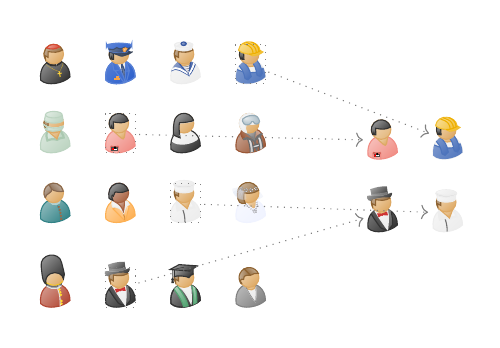
\begin{tikzpicture}
   \tikzstyle{agent}=[draw,fill=magenta!20,minimum height=7mm,minimum width=20mm,node distance=12mm]]
   \tikzstyle{sel}=[draw]

   \matrix (pop) [matrix of nodes,row sep=3mm,column sep=4mm] {
      \node [priest] {} ; &
      \node [conductor] {} ; &
      \node [sailor] {} ; &
      \node (p2) [builder] {} ; \\
      \node [surgeon] {} ; &
      \node (p1) [nurse] {} ; &
      \node [nun] {} ; &
      \node [pilot] {} ; \\
      \node [charlie] {} ; &
      \node [alice] {} ; &
      \node (p4) [chef] {} ; &
      \node [bride] {} ; \\
      \node [guard] {} ; &
      \node (p3) [groom] {} ; &
      \node [graduate] {} ; &
      \node [bob] {} ; \\
   } ;
   \draw [gray,dotted] (p1.north west) rectangle (p1.south east) ;
   \draw [gray,dotted] (p2.north west) rectangle (p2.south east) ;
   \draw [gray,dotted] (p3.north west) rectangle (p3.south east) ;
   \draw [gray,dotted] (p4.north west) rectangle (p4.south east) ;
   \matrix [right=of pop,matrix of nodes,row sep=3mm,column sep=4mm] {
      \node (s1) [nurse] {} ; &
      \node (s2) [builder] {} ; \\
      \node (s3) [groom] {} ; &
      \node (s4) [chef] {} ; \\
   } ;
   \draw [dotted,gray,->] (p1) -> (s1) ;
   \draw [dotted,gray,->] (p2) -> (s2) ;
   \draw [dotted,gray,->] (p3) -> (s3) ;
   \draw [dotted,gray,->] (p4) -> (s4) ;
\end{tikzpicture}
\end{document}
